\subsection{Registrarse}

\begin{figure}[ht]
\centering
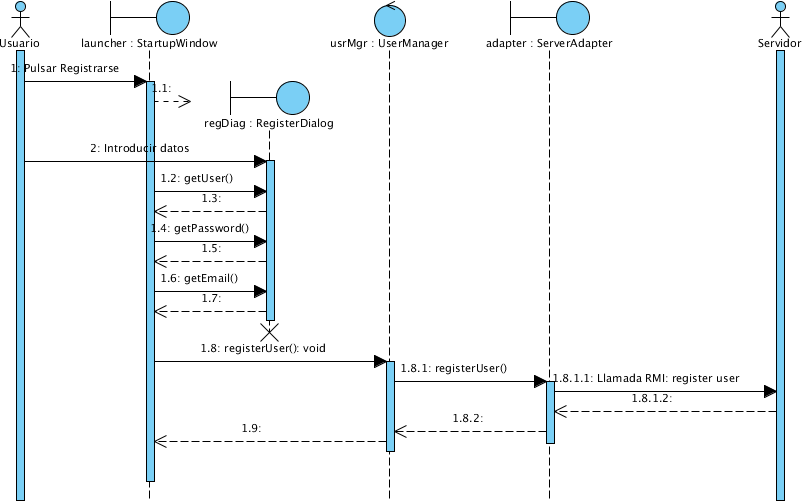
\includegraphics[scale=0.6]{img/ch03devel-register.png}
\caption{Diagrama de secuencia de ``Registrarse''}
\end{figure}

Cuando el usuario pulse el botón ``Registrarse'', se mostrará el diálogo de
registro \texttt{RegisterDialog}. Este diálogo se ejecutará de manera modal,
por lo que bloqueará el flujo de ejecución en la aplicación principal hasta que
el usuario lo complete.

A continuación, la aplicación llamará a la función correspodiente en el gestor
de usuarios para llevar a cabo el registro. Éste a su vez realizará la llamada
RMI a través del \texttt{ServerAdapter}.

Este caso de uso no provoca cambios en el estado interno del gestor de usuarios.
